\documentclass[12pt,a4paper]{article}

\usepackage[fleqn]{amsmath} % This package with the fleqn option aligns equations to the left
\setlength{\mathindent}{0pt} % Set indentation from the left margin

\usepackage{amssymb} % Required for math symbols
\usepackage{graphicx} % Required for inserting images
\usepackage{geometry}

\usepackage{stmaryrd}

\usepackage{amsmath, amssymb, amsthm}
\usepackage{xeCJK}

\usepackage{amsthm}
\usepackage{fullpage}
\usepackage{hyperref}

\usepackage{CJKutf8}


\usepackage[backend=biber, style=authoryear, citestyle=authoryear]{biblatex}
\addbibresource{references.bib}

\geometry{a4paper, margin=1in}



\usepackage{listings}
\usepackage{color}

\definecolor{codegreen}{rgb}{0,0.6,0}
\definecolor{codegray}{rgb}{0.5,0.5,0.5}
\definecolor{codepurple}{rgb}{0.58,0,0.82}
\definecolor{backcolour}{rgb}{0.99,0.99,0.99}

\lstdefinestyle{mystyle}{
    backgroundcolor=\color{backcolour},   
    commentstyle=\color{codegreen},
    keywordstyle=\color{magenta},
    numberstyle=\tiny\color{codegray},
    stringstyle=\color{codepurple},
    basicstyle=\ttfamily\footnotesize,
    breakatwhitespace=false,         
    breaklines=true,                 
    captionpos=b,                    
    keepspaces=true,                 
    numbers=left,                    
    numbersep=5pt,                  
    showspaces=false,                
    showstringspaces=false,
    showtabs=false,                  
    tabsize=2
}
\lstset{style=mystyle}


\begin{document}
\begin{CJK}{UTF8}{ipxm}

{
    \title{
        
\includegraphics[width=0.34\textwidth]{/Users/mlnick/documents/images/tsukuba-logo.png} \\
        \textbf{ソフトコンピューティング基礎論} \\
        \vspace{3mm}    
        レポート課題 1
    }
    
    \author{Mamanchuk Mykola, SID.202420671}
    \date{\today}
}
    
\maketitle



\setlength{\fboxsep}{0pt} % Removes padding around the image
\setlength{\fboxrule}{0.5pt} % Sets the thickness of the border

\section*{3囚人問題 (M. Gardner, 1959)}

\subsection*{問題の概要}
3人の囚人 A, B, C は、それぞれ別々の独房に収容され、死刑宣告を受けています。しかし、裁判所はランダムに1名に恩赦を与えると決定しました。看守は恩赦される囚人の名前を知っていますが、囚人たちは知りません。

囚人 A は看守に次のように依頼します：
\begin{quote}
「私自身についての情報は要りません。もし囚人 B が恩赦ならば、囚人 C の名前を、囚人 C が恩赦ならば囚人 B の名前を教えてください。もし私が恩赦で、B も C も死刑になる場合は、B と C のうちどちらかをランダムに選んで名前を教えてください。」
\end{quote}

看守は「B は死刑になる」と答えます。これを受けて囚人 A は、
\begin{quote}
「つまり、死刑になるのは私か C ということだ。死刑の確率が $2/3$ から $1/2$ に下がった。」
\end{quote}
と考え、喜びます。ここで、囚人 A の考えが正しいかを理論的に検討します。

\subsection*{初期状況の確率}
どの囚人が恩赦されるかは均等に決まると考えると、
\[
P(A \text{が恩赦}) = \frac{1}{3},\quad P(B \text{が恩赦}) = \frac{1}{3},\quad P(C \text{が恩赦}) = \frac{1}{3}.
\]
よって、各囚人が死刑になる確率は
\[
P(\text{死刑}) = \frac{2}{3}.
\]

\subsection*{看守の発言と条件付き確率}
A の依頼により、看守は B または C のうちどちらかの名前を A に教える必要があります。それぞれの場合を考えます。

\begin{itemize}
    \item \textbf{ケース1:} $B$ が恩赦の場合\\
    この場合、指示に従い、看守は必ず $C$ の名前を伝えなければなりません。したがって、看守が「Bは死刑」と言う確率は $0$ です。
    
    \item \textbf{ケース2:} $C$ が恩赦の場合\\
    この場合、看守は必然的に $B$ の名前を告げます。よって、この場合の確率は $1$ です。
    
    \item \textbf{ケース3:} $A$ が恩赦の場合\\
    この場合、B と C は共に死刑となるので、看守は B と C のどちらかの名前をランダムに選びます。よって、選ばれる確率は $1/2$ です。
\end{itemize}

看守が「Bは死刑」と答える確率は、各場合の事前確率と条件付き確率の積の和で与えられます。

\begin{figure}[ht]
    \centering
    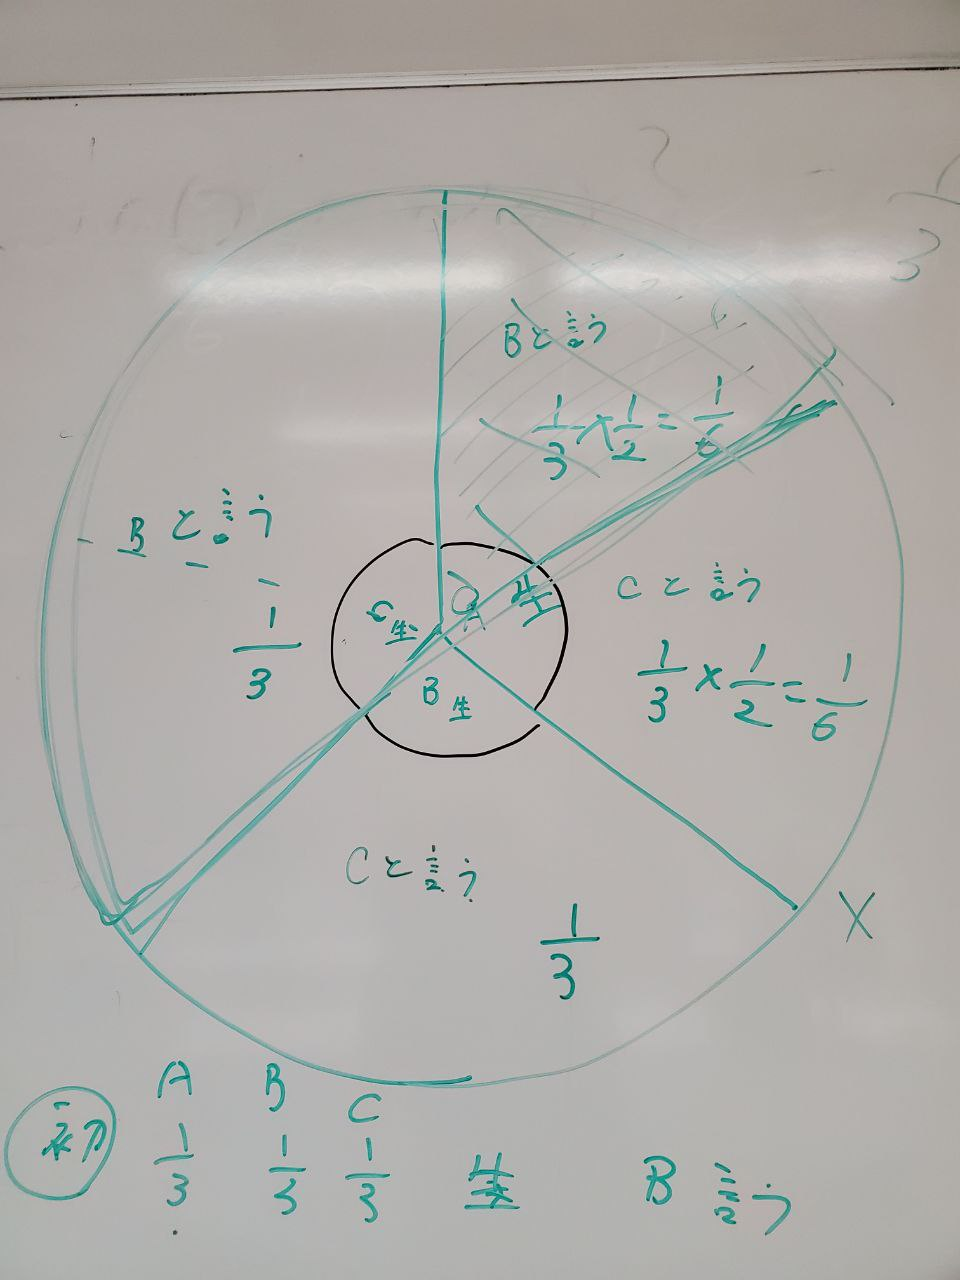
\includegraphics[width=0.5\textwidth]{graph_11.jpg}
    \caption{Three Prisoners Problem Diagram}
    \label{fig:3prisoners}
\end{figure}

\subsubsection*{計算}
\begin{enumerate}
    \item \textbf{ケース3 ($A$ が恩赦の場合):}
    \[
    P(A \text{恩赦}) = \frac{1}{3},\quad P(\text{「Bは死刑」} \mid A \text{恩赦}) = \frac{1}{2}.
    \]
    よって、この枝の合成確率は
    \[
    \frac{1}{3} \times \frac{1}{2} = \frac{1}{6}.
    \]
    
    \item \textbf{ケース1 ($B$ が恩赦の場合):} 
    \[
    P(B \text{恩赦}) = \frac{1}{3},\quad P(\text{「Bは死刑」} \mid B \text{恩赦}) = 0.
    \]
    
    \item \textbf{ケース2 ($C$ が恩赦の場合):}
    \[
    P(C \text{恩赦}) = \frac{1}{3},\quad P(\text{「Bは死刑」} \mid C \text{恩赦}) = 1.
    \]
    よって、この枝の合成確率は
    \[
    \frac{1}{3} \times 1 = \frac{1}{3}.
    \]
\end{enumerate}

これらを合わせると、
\[
P(\text{「Bは死刑」}) = \frac{1}{6} + 0 + \frac{1}{3} = \frac{1}{6} + \frac{2}{6} = \frac{3}{6} = \frac{1}{2}.
\]

\subsection*{ベイズの定理による確率更新}
看守の「Bは死刑」という発言があったとき、囚人 A が恩赦される条件付き確率は、次のように求められます：
\[
P(A \text{恩赦} \mid \text{「Bは死刑」}) = \frac{P(A \text{恩赦}) \cdot P(\text{「Bは死刑」} \mid A \text{恩赦})}{P(\text{「Bは死刑」})} = \frac{\frac{1}{3} \times \frac{1}{2}}{\frac{1}{2}} = \frac{1}{3}.
\]
また、囚人 C が恩赦される条件付き確率は、
\[
P(C \text{恩赦} \mid \text{「Bは死刑」}) = \frac{\frac{1}{3} \times 1}{\frac{1}{2}} = \frac{2}{3}.
\]

\subsection*{結論}
看守の発言「Bは死刑」によって、囚人 A の恩赦される確率は $\frac{1}{3}$ のままであり、囚人 C の恩赦される確率は $\frac{2}{3}$ に上がります。囚人 A は、自分の生存確率が $\frac{1}{2}$ にまで上がったと誤解しましたが、実際には条件付き確率を考えるとその解釈は誤りであることが分かります。この現象は、モンティ・ホール問題と似た条件付き確率の直感に反する面白い例です。



%\subsection*{Listing .java}
%\begin{lstlisting}

%\end{lstlisting}

\section*{参照}
\begin{enumerate}
    \item \textbf{Mamanchuk N., University of Tsukuba}, Github, \today. Available online: \url{https://github.com/RIFLE}
\end{enumerate}


\end{CJK}
\end{document}
